\documentclass[11pt ,a4paper]{article} 
\usepackage{graphicx}
\usepackage[a4paper, total={6.5in, 9in}]{geometry}
\usepackage{cite}
\usepackage{amsmath}
\usepackage{graphicx}
\usepackage{mathtools}
\usepackage{hyperref}
\begin{document} 
\title{Neutrino Oscillations: From Homestake Experiment To The Discovery of Non-Vanishing Reactor Mixing Angle. Connections with Physics Beyond The Standard Model}
\author{Ken Lee\\ ID:2565 3784\\ School of Physics and Astronomy\\ University of Southampton\\ kkl2g12@soton.ac.uk}
\date{\today}
\maketitle
\begin{abstract}
Ever since the Homestake experiment were able to first verify that neutrino does oscillates which then proposed that the standard model may need some expansion or new theories to include the mass of Neutrino. First we may discuss some of the experiment in the last 2 decade or so where neutrino experiment were able to obtained better resolution than ever before in detecting and measuring the mixing angles of neutrino oscillation. With the recent discovery of theta-13 is non-zero, type-1 see-saw mechanism may seen as the best possible candidate in explaining neutrino mass. Grand Unified Theory may be the possible next step after Standard Model as with the LHC restarting soon for even higher energy, neutrino oscillation may be the clue some of these next step beyond the standard model.
\end{abstract}
\section*{Neutrino Physics}
The existence of Neutrino, \(\nu \) is first proposed by Austrian physicist Wolfgang Pauli in 1930's to explain the missing energy in a radioactive decay process, beta decay. Pauli proposed that this particle has no charge and neutrino were later discovered by Clyde Cowan and Fred Reines from a Nuclear reactor in 1956.\cite{king07} Later, neutrino were discovered as an integral part of Standard Model as the fundamental building block of matter. The three flavour of neutrino that we know today are subsequently first observe experimentally by the Homestake experiment.
\subsection*{Homestake Experiment}
The very first experimental observation of neutrino oscillation were first discovered by two american scientist, Raymond Davis Jr and John Bahcall in an underground experiment in the late 1960's. In the experiment, only one-third of the predicted neutrino from the core of Sun were detected \cite{king07}. This was the first instance where physicist are suspecting that the solar neutrinos, \(\nu_e \) detected from the Sun might be changing into something else or later known as Neutrino Oscillation.
\subsection*{Neutrino Oscillation}
In 1957, first proposed by Bruno Pontecorvo a Russian physicist where a neutrino can be created with a specific lepton flavour can later be measured to have a different flavour.\cite{bruno}\cite{wolf} This flavour changing is analogous to Kaon and the occurrence of neutrino oscillation suggest the neutrino are not actually massless as first initially predicted by the Standard model. Later experiment and observation has proved that this flavour changing or Neutrino oscillation does occurs and neutrino does have a absolute mass scale. With Pontecorvo's idea, the exact mechanism to explain neutrino oscillation was later proposed by three physicist, Mikheyev, Smirnov and Wolfenstein where involvement of resonant enhancement of neutrino oscillation due to matter effects is known as the MSW effect.\cite{massmodel} Neutrino Oscillation are also later discovered that the flux of the electron neutrino from the Sun, \(\nu_e \) are related to the azimuth angle or mixing angles as known within the physicist in the Super-Kamiokande experiment in 1998.\cite{king07} With experiments such as Super-Kamiokande and Sudbury Neutrino Observatory in the late 1990's, neutrino physics has gain much more momentum where research are heavily involved in this area of neutrino physics in the last two decades.
\subsection*{Motivation of neutrino oscillation in beyond the Standard Model}
Neutrino oscillation occurs because of the reason that neutrino has definite mass which contradicts with the Standard Model. This contradiction implies that the current Standard Model we have is incomplete and may need some extension to it or new physics is needed that is beyond the Standard Model. With the development of the last two decades in the field of Neutrino physics where Cherenkov detector are getting better resolution that is vital in determine the non-vanishing vector, the \(\theta_{13} \) which may subsequently provide clue on the absolute scale of the neutrino mass.
\section*{Neutrino in the Standard Model}
The three neutrino flavours in the Standard model are massless for three independent reasons:-
\begin{itemize}
	\item there are no right-handed neutrino\(\nu_R \) in the Standard Model,
	\item there are only Higgs Doublets(\(H\textsuperscript{+} \), \(H\textsuperscript{0} \) ),
	\item the theory is renormalizable.\cite{king07} 
\end{itemize}
Neutrino are massless in the Standard Model because there are only left-handed neutrino in the SM, this means that neutrinos pass through space without interacting with Higgs fields as it does not interact with the Higgs field. Some physicist proposed that the right-handed neutrino may have very small mass compared to the left-handed neutrino up to 1000 times lighter than left-handed, because of this theories such as see-saw mechanism are gaining favour in explaining right-handed neutrino with the recent development of LHC failed to detect new particle after the Higgs.

The second reason is that since the standard model predicts neutrino are massless, the background Higgs field \(H^0 \) is incapable of flipping a left-handed neutrino into a right-handed neutrino or its conjugates. But with Higgs doublet (\(H^+, H^0 \)), the neutrino can flip into a right-handed neutrino but not its conjugate. With Higgs triplets (\(H^{++}, H^+, H^0\)), the flipping of left-handed into right-handed or conjugate maybe be possible. This would be clearer if we were to determine the neutrino are whether Dirac or Majorana.\cite{electroweak}

The third reason is the renormalisation condition of the Standard Model where the interaction of the theory is is generated by particle exchange. The interaction of left-handed neutrino are considered as "contact interactions" rather than exchange which makes neutrino oscillation are non-renormalisablem within the boundary of the current Standard Model.\cite{king07}
 \begin{figure}[h]
	\centering
		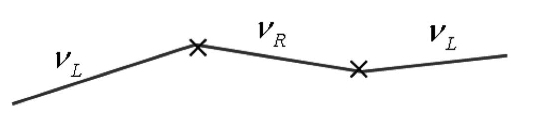
\includegraphics{righthand.png}
	\caption{Assuming right-handed does exist, then the neutrino would jiggle as it move through space, the length of \(\nu_R \) would be discuss later where it would represent the possible mass of right-handed neutrino. image taken from\cite{king07}}
\end{figure}
\section*{Dirac or Majorana - mass nature of neutrino}
The Standard Model describe the origin of mass of most of the particle in the Standard Model but the Higgs field is not directly responsible for the mass of neutrino due to the interaction within the Standard Model. 

For mass to exist, each particle must be constitute of a left-handed and a right handed "parts" so that it would jiggle along as it travels through the Higgs fields. If a particle travels through a field without interacts with it then it would just pass through in a straight at the speed of light which means that the particle is massless. However neutrino as observed from experiment it has mass therefore we would need an explanation of how the neutrino travels through the field in order to explain its mass.\cite{constraint}
\subsection*{Majorana}
If neutrino are Majorana fermions, the neutrino would probably have a mass term from the Lagrangian of the Standard Model,\cite{constraint}
\begin{equation}
\mathcal{L}= -\frac{1}{2}\overline{\nu_L^c}M_{\nu}\nu_L+H.c.= \frac{1}{2}\nu_L^TC^{-1}M_{\nu}\nu_L+H.c., 
\end{equation}
where \(M_{\nu} \) is a complex symmetric 3x3 matrix. This term can be explain directly via Type-II see-saw mechanism and also effectively generated via type I and III. \cite{constraint} This idea is much more favourable within physicist as the idea of Majorana mass is linked heavily with see-saw Mechanism where it is more likely to explain the mass of neutrino with the idea that right-handed neutrino maybe much more smaller than its left-handed counterpart.
\subsection*{Dirac}
If neutrino are Dirac particle, assuming that the total lepton number is conserved and the existence of right-handed neutrino, \(\nu_R \) the mass term from the Lagrangian of the Standard Model would be,\cite{constraint}
\begin{equation}
\mathcal{L}=-\overline{\nu_R}M_D\nu_L+H.c.,
\end{equation}
where \(M_D \) is an arbitrary complex 3x3 matrix.\cite{constraint} If neutrino are Dirac particle indeed then the concern of Charge Parity(CP) would not be a concern in the mass nature of neutrino. Though this option is getting out of favour due to recent result supporting the idea that neutrino maybe Majorana in nature.
\section*{Lepton Mixing Matrix assuming Right-handed Neutrino does exist in Standard Model}
To start the discussion of neutrino oscillation, it would be best first introduced the lepton mixing matrix of the Standard Model by assuming right-handed neutrino exist in the standard model. This would lead to a mixing matrix which shows the relation between the three different neutrino flavour. This mixing matrix is obtained by assuming that the neutrino are Majorana which lead to an additional CP violation phase in the matrix and of course adding a right-handed neutrino to the system.\cite{king07}
	\begin{equation}
	\begin{pmatrix}
	\nu_e\\\nu_{\mu}\\\nu_{\tau} 
	\end{pmatrix}
	=\begin{pmatrix}
	U_{e1}&U_{e2}&U_{e3}\\U_{\mu1}&U_{\mu2}&U_{\mu3}\\U_{\tau1}&U_{\tau2}&U_{\tau3}
	\end{pmatrix}
	\begin{pmatrix}
	\nu_1\\\nu_2\\\nu_3
	\end{pmatrix}
	\end{equation}
The 3x3 matrix above can be express as follow as a Lepton mixing matrix with a Majorana term at the back
\begin{equation}
U_{MNS}=
\begin{pmatrix}
c_{12}c_{13}&s_{12}c_{13}&s_{13}e^{-i\delta}\\
-s_{12}c_{23}-c_{12}s_{13}s_{23}e^{i\delta} & c_{12}c_{23}-s_{12}s_{13}s_{23}e^{i\delta} &c_{13}s_{23}\\
s_{12}s_{23}-c_{12}s_{13}c_{23}e^{i\delta} &-c_{12}s_{23}-s_{12}s_{13}c_{23}e^{i\delta} & c_{13}c_{23}
\end{pmatrix}
\begin{pmatrix}
e^{i\alpha_1/2}&0&0\\0&e^{i\alpha_2/2}&0\\0&0&1
\end{pmatrix}
\end{equation}
\cite{globalfit} can be rewritten as
\begin{equation}
U_{MNS}=
\begin{pmatrix}
1&0&0\\0&c_{23}&s_{23}\\0&-s_{23}&c_{23}
\end{pmatrix}
\begin{pmatrix}
c_{13} & 0 & s_{13}e^{-i\delta}\\0&1&0\\-s_{13}e^{i\delta}&0&c_{13}
\end{pmatrix}
\begin{pmatrix}
c_{12}&s_{12}&0\\-s_{12}&c_{12}&0\\0&0&1
\end{pmatrix}
\begin{pmatrix}
e^{i\alpha_1/2}&0&0\\0&e^{i\alpha_2/2}&0\\0&0&1
\end{pmatrix}
\end{equation}
where \(s_{ij}=\sin{\theta_{ij}} \) and \(c_{ij}=\cos{\theta_{ij}} \),  \(\delta \) is the phase related to the CP violation of the Standard Model. The first matrix is related to the atmospheric mixing, \(\theta_{23} \) with the third matrix correlated to the solar mixing, \(\theta_{12} \). The second matrix is related to the reactor mixing angle, \(\theta_{13} \) and this value is the main concern of physicist as it may shed light on the nature of neutrino mass and neutrino oscillation. Equation 5 in fact is the expression of the Lepton mixing matrix with parameterisation of three Euler Rotations\cite{massmodel}\cite{constraint} hence the figure 2.

\section*{Mixing angles}
\subsection*{Tri-bimaximal mixing}
The maximal mixing angles, \(\theta_{12}, \theta_{13}, \theta_{23} \) hence the name tri-bimaximal mixing angles, is one of the early names used in neutrino oscillation in relation of the 3 neutrino.\cite{tip} The angles for neutrino oscillation is the early days are known as tri-bimaximal mixing due to the accuracy of determine these values after the Kamiokande experiment era.\cite{trip}
\subsection*{\(\theta_{12} \), \(\theta_{23} \) and \(\theta_{13} \)}
Current going around the world in the area of neutrino experiments, Physicist are trying hard to determine the best possible value for the mixing angles as it is vital that these value are obtain accurately as these will determine the nature of neutrino whether they are Majorana or Dirac. These result might also provide clue as to help physicist to determine the absolute mass of neutrino as currently there are no way we could measure directly the neutrino mass. These value would be some of the clue we need in explaining neutrino mass especially the nature of right-handed neutrino. The table below are some of the parameter in the Lepton Mixing angles determined via experiments or observations. \cite{theta130}
\begin{table}[htdp]
\begin{center}
\begin{tabular}{|p{2cm}|p{2.2cm}|p{2.3cm}|p{2.3cm}|p{2.3cm}|p{2.3cm}|}
\hline
Parameter & \(\delta m^2/10^{-5} \)e\(V^2 \) & \(\sin^2\theta_{12}\)& \(\sin^2\theta_{13}\)& \(\sin^2\theta_{23}\)&\(\delta m^2/10^{-3} eV^2 \)\\ \hline
Best fit & 7.85 & 0.306 (0.312) & 0.021 (0.025) & 0.42 & 2.35\\ \hline
1\(\sigma \) range & 7.32-7.80 & 0.291-0.324 (0.296-0.329) & 0.013-0.028 (0.018-0.032) & 0.39-0.50 & 2.26-2.47 \\ \hline
\end{tabular}
\end{center}
\label{default}
\caption{the best fit values for the mass mixing parameters, parenthesis are value shifted by +0.006 or +0.004 \cite{theta130}}
\end{table}%

From the table, the value of \(\theta_{12} \) and \(\theta_{23} \) is much more obvious and this allow experiment to determine the value much easily. A rough visual representation of these angles with its unitary matrix can be seen from figure 2.
\begin{figure}[htbp]
\begin{center}
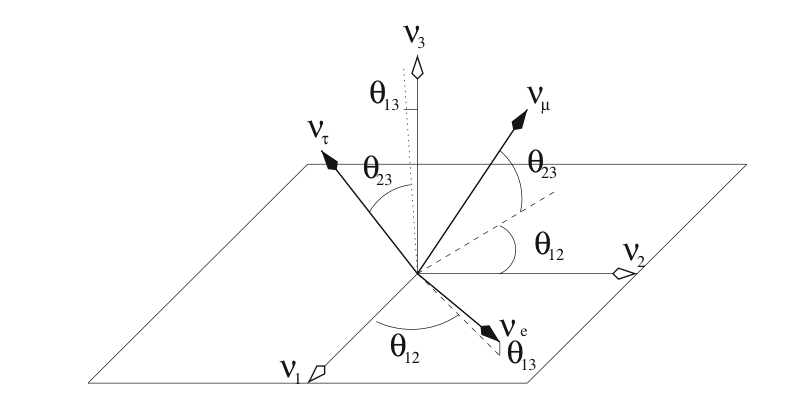
\includegraphics{theta.png}
\caption{Euler angles of neutrino weak eigenstates \(\nu_e, \nu_{\mu}, \nu_{\tau} \)  and neutrino mass eigenstates \(\nu_1, \nu_2, \nu_3 \) in terms of mixing angles \(\theta_{12}, \theta_{13}, \theta_{23} \) ignoring CP violating phase, image from\cite{massmodel}}
\label{default}
\end{center}
\end{figure}

The first two mode of oscillation, \(\theta_{12} \) and \(\theta_{23} \) are determined via the observation of solar and atmospheric neutrinos which are more of observable experiments. However \(\theta_{13} \) the neutrino oscillation of muon are more commonly produced in the particle accelerator\cite{kamiokande} which are more difficult to be obtained and the value is predicted to be much smaller than the previous two modes where the resolution of the Cherenkov detector has to be improve greatly where currently most work are on this area.
\subsection*{Non-vanishing \(\theta_{13} \)}
Since the extensive research of neutrino started in the late 90's, \(\theta_{13} \) was always assumed to be zero as clearly seen from figure 2 that it is a good approximation due to the fact that \(\theta_{13} \) value is about 10 magnitude smaller than \(\theta_{12} \) and \(\theta_{23} \). However as Cherenkov detector which are responsible for detecting neutrino are getting better as years goes by, experimental results has shown that \(\theta_{13} \) may not be none zero as the resolution of the detectors improves. With \(\theta_{13} \) is non-vanishing, the CP-violation of the standard model comes into place as the total lepton number is not conserved within the boundaries of the Standard Model. As to the problem of Charge Polarity Violation within the Standard Model, It could lead to more topic to discussion but for the matter of neutrino oscillation, we would put aside it for this dissertation.\cite{theta130}\cite{global fit}
\section*{Detection of Neutrino}
The main tool for detecting these relatively neutral particle are known as Cherenkov detector. These are basically large medium of liquid surrounded by hyper sensitive photodiode in an enclose container and are normally located few hundred meter underground. they are more commonly they are filled with pure heavy water or medium with high density of nuclei. The neutrino will collide inelastically with a nuclei and hopefully that the collision would produce enough energy that will be emitted as a photon via Cherenkov radiation where particles appears to travel faster than the speed of light of the medium producing blue flashes as commonly observe in nuclear reactor.\cite{kamiokande}

The source of neutrino can be from two source, one from the nuclear fusion in the core of the Sun which are normally observed by Observatory such as Sudbury Neutrino Observatory(SNO).Another way of producing neutrino are from the radioactive activity at a nuclear reactor normally beta decay such as from the JHF to Super-Kamiokande experiment or neutrino from particle accelerator such as the LHC to OPERA. 

Although Homestake experiment were the first to speculate neutrino oscillation, it took more than 3 decades before in depth study can be done due to the resolution of Cherenkov detector were limited to further study neutrino. The Super Kamiokande in 1998 were among the first experiment that a Cherenkov detector were able to achieve a better resolution than ever before and subsequently speed up the research in the area of Neutrino physics. \cite{wolf}

Considering a 2 state probability oscillation of muon and tau neutrino,\cite{king07}
\begin{equation}
P(\nu_{\mu}\to\nu_{\tau})=\sin^2{2\theta_{23}}\sin^2{(1.27\Delta m^2_{32}\frac{L}{E})}
\end{equation}
Equation shown above is the probabilistic equation used in measuring these neutrino. By comparing the statistical data and theoretical data, this allows physicist to verify the claims about neutrino oscillation.
\section*{Experimental Observation}
Experiment around the world in the area of neutrino physics are generally categorised into 2 kind of experiment, accelerator based experiment and Observatory. Observatory kind of experiment such as ICECUBE, KEK and SNO are mostly studying the oscillation of atmospheric and solar neutrino and usually conduct over a longer period as collision of neutrino are of low probability events. Accelerator based experiment can be meant that it is from a particle accelerator or from nuclear reactor where neutrino are common produced and where most of the difficult part of neutrino physics are conducted. However they are not limited as mentioned as there are experiments such as neutrinos double beta decay which focus more towards the end spectrum of beta decay where high resolution detector are needed.
\cite{theta130}
\section*{Possible Theories to Explain Neutrino Oscillation}
This neutrino flavour changing mechanism more commonly known as neutrino oscillation has a few concepts that may explain it with each theory has its unique condition to it. There are Type I and Type II see-saw mechanism, double see-saw mechanism, Form Dominance and Sequential Dominance. However with the recent result of the non-zero of \(\theta_{13} \), Type I see-saw mechanism is the most prominent candidate in explaining neutrino oscillation. There may have some proposed theory that was not mentioned but at the end of the day is that the experimental result supports the theory which in the next decade or so a solid theory should be able to explain fully the neutrino oscillation and subsequently shed some light on the absolute mass of neutrino.\cite{massmodel}\cite{king07}
\subsection*{See-saw Mechanism}
This idea of a see-saw can be conceptualise as a pair of pendulum in a resonance experiment where the oscillation of the single pendulum can cause the other pendulum to oscillates. Analogously this can be applied to neutrino oscillation, and the mass of the pendulum in this case would be the mass of neutrino which explains the importance the neutrino can shed light on the neutrino mass. It is speculated that the right-handed neutrino or the counter part of the left-handed neutrino which yet to be confirmed can be hundreds or thousands time lighter than the left-handed neutrino. Because of this assumption, this would explain why neutrino are expected to be massless as left-handed neutrino travels thousands times more than its counter part as it travels through space.\cite{king07}\cite{massmodel} There are few kind of see-saw mechanism, type-1 referring to lighter right-handed, type-2 mostly about heavier right-handed and other proposed. However Type-1 see-saw mechanism is favour much upon.
\cite{chen}
\subsection*{The "counter part" of left-handed neutrino}
As the previously the "opposite" of the left-handed neutrino was not specify as it could be anti-neutrino that would the the conjugate of the left-handed neutrino or right-handed neutrino, \(\nu_R \) which means it would be Dirac. On the note of the anti-neutrino, it could be the left-handed anti-neutrino, \(\nu_{L}^C \) or right-handed anti-neutrino where this will lead into the discussion of Majorana mass. However the recent result is more favourable towards Majorana, therefore the focus would more towards conjugate of the left-handed neutrino.
\subsection*{Link to Leptogenesis/Baryogenesis}
Baryon are translated as heavy particle which are the particle that made up matter in the universe.\cite{}Some physicist speculate that leptogenesis may be the clue as the origin of matter in this universe came from. Although The discovery of Higgs boson is able to prove the origin of the mass of matter\cite{OriMatter} come from but the creation or origin of matter is yet to be determined. The absolute mass of neutrino and neutrino oscillation are needed to be understood first as we need a complete picture of the Standard Model. As of yet, physicist has yet have a absolute result on the neutrino mass which Higgs was failed to explained mass of neutrino as Higgs on interacts with left-handed neutrino. However with the progress of physics beyond the Standard Model the last few decades goes, within the next few decades or so we may have some solid physics in explaining these problems so these things are yet to be end of it..
\cite{dibari}
\subsection*{Grand Unified Theory}
The mass of the right-handed neutrino or the conjugates is suspected to be slight lower than the planck constant which means slight below the GUT scale. \cite{} This may mean that the next generations of particle accelerator which are more powerful than the LHC may be able to verify some theory that physicist proposed.\cite{king07}
\section*{Ongoing Experiments}
Most of the neutrino experiment currently are focusing on obtaining a better accuracy of the mass squared splitting including the sign between neutrino flavour. Also to obtain a more accurate value of the mixing angles especially \(\theta_{13} \) since the recent experiment agree that it is non-zero\cite{theta130} With the new neutrino experiment such as KATRIN which will be online by 2015 as one of the accelerator based neutrino experiment\cite{katrin}, we could come closer in solving the nature of neutrino oscillation and subsequently able to determine the absolute mass of neutrino.
\section*{Conclusion}
Neutrino oscillation first proposed during the Homestake experiment as the expected solar neutrino was only one third which then lead on that neutrino actually comes in 3 different flavour, \(\nu_e, \nu_{\mu}, \nu_{\tau} \) and the idea of neutrino undergoes oscillation. This shown that the Standard Model was imperfect as neutrino oscillation shows that neutrino need to have mass where within the Standard Model it was assumed massless and this definitely means that the Standard Model requires modifications or extensions or maybe new theory as there are things more to be studied upon beyond the Standard Model. Though the see-saw mechanism was not explain in depth due to lack in understandings and its complicated mathematics as understanding of the Standard Model needed to be comes first as the mathematics involved revolve around expanding the Standard Model.
\bibliography{reference}{}
\bibliographystyle{plain}
\nocite{*}
\end{document}